\chapter{Interferometry, Calibration \& Polarimetry}
\label{chapter:interferometry}

In this Chapter I wished to build a formalism around wide-field, polarized interferometric measurements that could be used throughout this work. Many traditional assumptions used in radio interferometry are broken in the case of the wide-field, fully-polarized, drift-scanning measurements native to interferometric EoR observations. In Section~\ref{sec:interferometry_vis}, I derive the equation describing the fundamental observable for an interferometer, called a ``visibility". Section~\ref{sec:interferometry_cal}, I describe calibration techniques relevant to this work and in Section~\ref{sec:interferometry_pol} I review some of the implications of the previous two sections for polarized measurements.

For a comprehensive review of interferometry from a more traditional perspective, see \cite{TMS}.

\section{The Visibility Equation}
\label{sec:interferometry_vis}

A radio interferometer (a term used interchangeably with ``interferometric array" for radio observations) is an ensemble of receiving elements, where each element's measurement is correlated with every other element's. The simplest case is a two-element interferometer, which we will focus on below. We assume (for now) that the elements are coplanar and identical.

\subsection{The Classical Visibility Equation}

Consider two receiving elements $i$ and $j$, separated by baseline vector $\vec{b}$. Suppose a plane wave of wavelength $\lambda$ is incident upon these elements, with direction of propagation $-\hat{s}$. The geometry of this interferometer is illustrated in Figure~\ref{fig:interferometry_2element}.

\begin{figure}
\centering
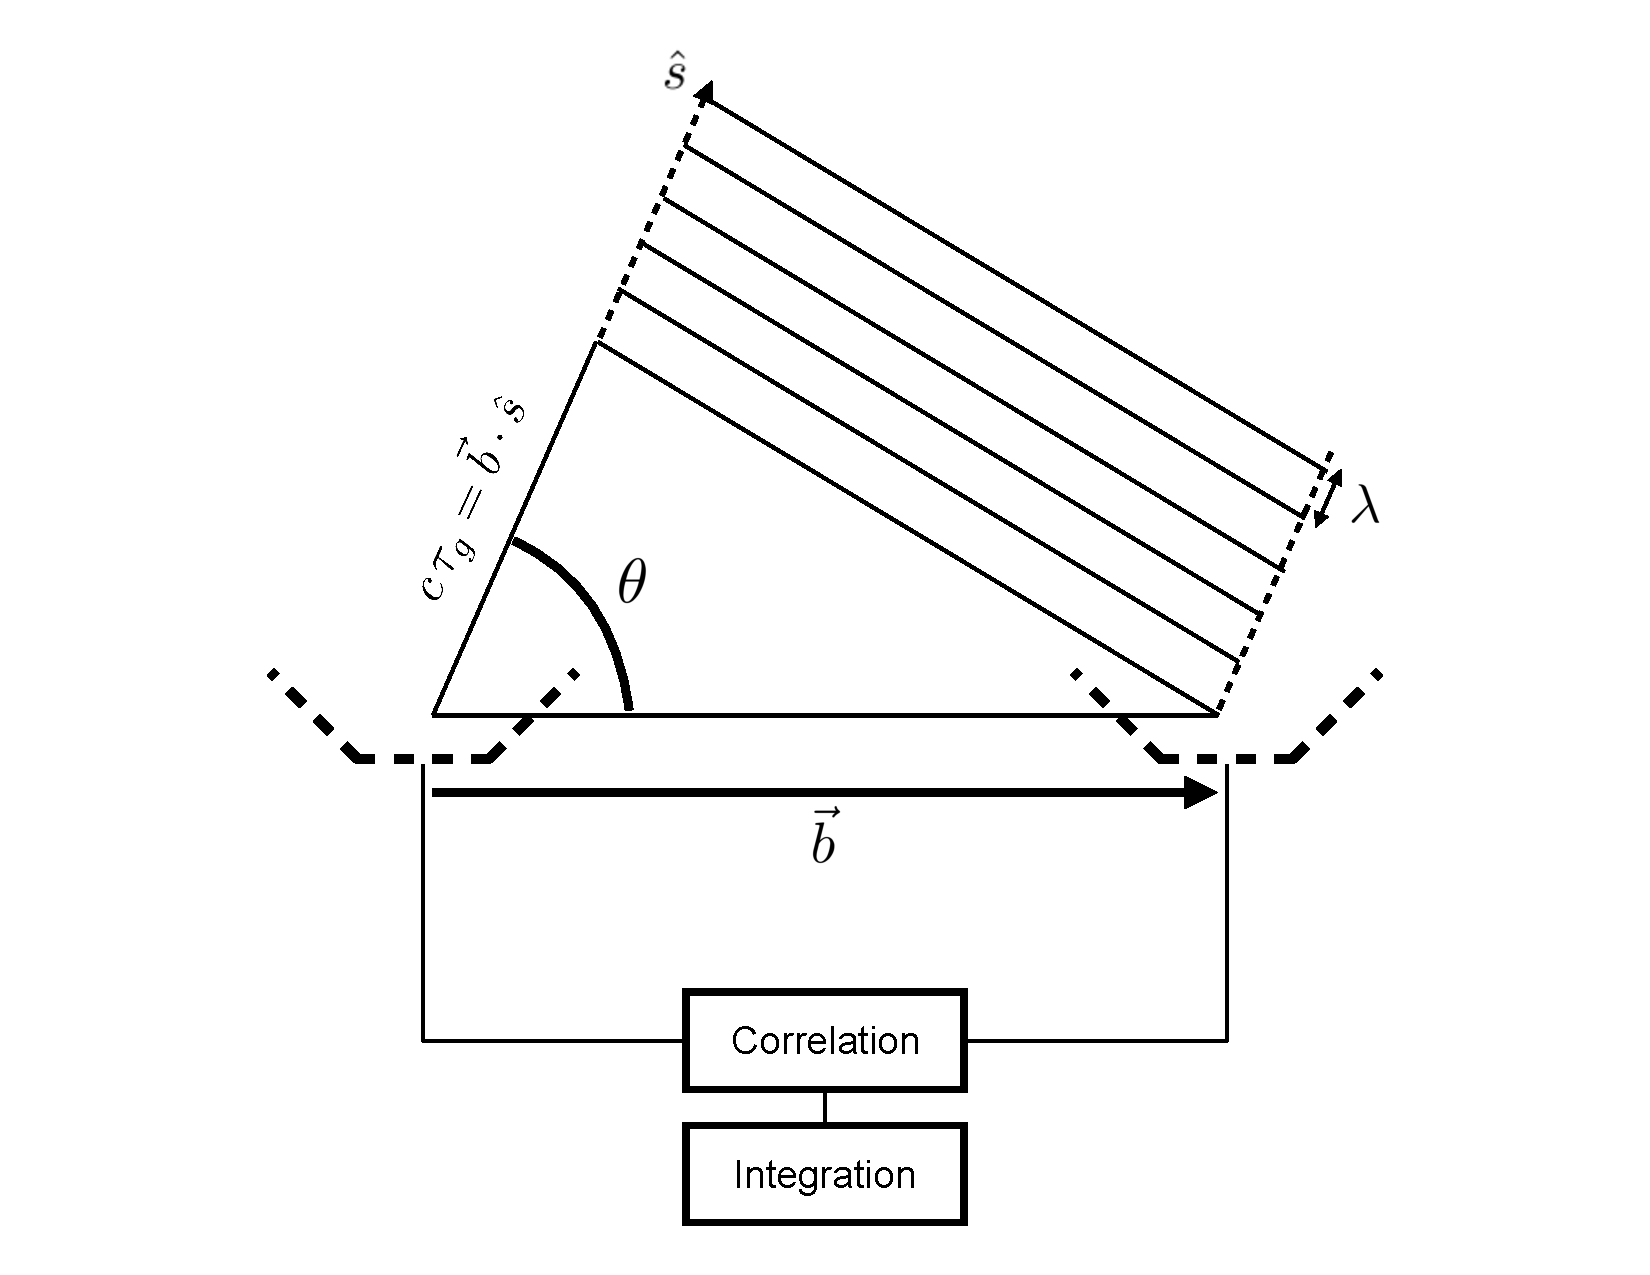
\includegraphics[width=0.9\textwidth]{chapters/interferometry/figures/visibility_explanation.pdf}
\caption{The geometry of a two-element interferometer, with a plane wave incident from direction $\hat{s}$.}
\label{fig:interferometry_2element}
\end{figure}

We can define the electromagnetic wave to have a frequency dependent phase, such that the electric field measured by element $i$ at time $t$ is

\begin{equation}
E_i = E_0 e^{-2\pi i \nu t}.
\end{equation}

The time difference between the arrival at $i$ and $j$ is called the ``geometrical delay", $\tau_g$:

\begin{equation}
\tau_g = \frac{\vec{b}\cdot\hat{s}}{c}
\end{equation}

and the electric field measured by element $j$ is

\begin{equation}
E_j = E_0 e^{-2\pi i \nu (t+\tau_g)}
\end{equation}

An interferometer is an instrument which correlates these electric fields together, integrating their product over some coherent time-scale. This correlation grants:

\begin{equation}
\langle E_i E_j^* \rangle 
= \lim_{T\rightarrow\inf}\frac{1}{2T}\int^T_{-T} E_i(t) E_j(t) {\rm d}t
= | E_0 |^2 e^{-2\pi i \nu \tau_g}
\end{equation}

where $e^{-2\pi i \nu \tau_g} = e^{-2\pi i \nu \vec{b}\cdot\hat{s}/c}$ is known as the ``fringe" term, due to its sinusoidal nature. We can generalize this relationship to include more than a single plane wave from direction $\hat{s}$. Many plane waves from all directions can be incident upon the interferometer at a given 

\subsection{The Measurement Equation}

% building the [classical] visibility equation in the unpolarized case
% pointing vs drift-scanning
% wide field effects
% rebuilding the visibility equation for widefield, polarized instruments
% Stokes visibilities

\section{Calibration Techniques}
\label{sec:interferometry_cal}

% basics of calibration for drift-scanning interferometers
% redundant calibration theory (more in polcal chapter)
% redundant vs imaging configurations
% CLEAN

\section{Instrumental Polarization}
\label{sec:interferometry_pol}

%%% Instrumental polarization:
% explore the matrix-formalized visibility equation
% DI leakage
% DD leakage